\documentclass[tikz, border=15pt]{standalone}
\usepackage{tikz}
\usetikzlibrary{arrows.meta, calc, patterns, decorations.pathreplacing}
\usepackage{amsmath, lmodern}
\usepackage[T1]{fontenc}

\begin{document}
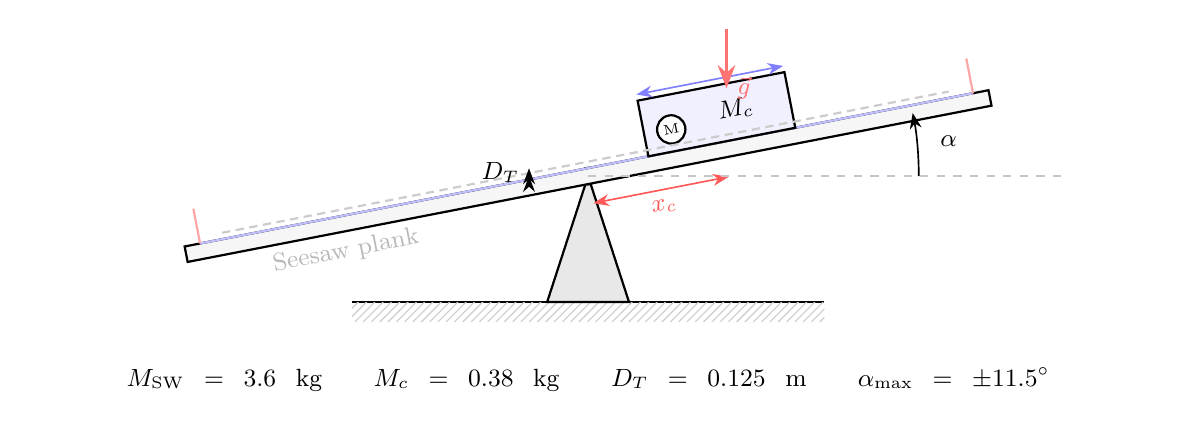
\begin{tikzpicture}[>=Stealth, thick]

  \def\tilt{11}
  \def\halflen{5.2}

  %%──────────────────────────────────────────────────────────────────────────
  %%  GROUND + PIVOT SUPPORT
  %%──────────────────────────────────────────────────────────────────────────
  \draw[thick] (-3.0, -1.6) -- (3.0, -1.6);
  \fill[pattern=north east lines, pattern color=gray!40]
    (-3.0, -1.85) rectangle (3.0, -1.6);

  %% Triangle pivot support
  \draw[fill=gray!18, thick] (-0.52, -1.6) -- (0.52, -1.6) -- (0, 0) -- cycle;
  \filldraw (0, 0) circle (3pt);

  %%──────────────────────────────────────────────────────────────────────────
  %%  BEAM + CART  (drawn in rotated frame)
  %%──────────────────────────────────────────────────────────────────────────
  \begin{scope}[rotate=\tilt]

    %% Beam (seesaw plank)
    \draw[fill=gray!7, thick] (-\halflen, -0.10) rectangle (\halflen, 0.10);

    %% Track surface
    \draw[blue!25, thick] ({-\halflen+0.2}, 0.10) -- ({\halflen-0.2}, 0.10);

    %% Cart body
    \draw[fill=blue!6, thick] (0.8, 0.10) rectangle (2.7, 0.82);

    %% Motor symbol
    \draw[fill=white, thick] (1.15, 0.38) circle (0.18);
    \node[font=\tiny, rotate=\tilt] at (1.15, 0.38) {M};

    %% Cart label
    \node[font=\small, rotate=\tilt] at (2.0, 0.48) {$M_c$};

    %% Rack (dashed line along track)
    \draw[gray!40, densely dashed] ({-\halflen+0.5}, 0.18) -- ({\halflen-0.5}, 0.18);

    %% Cart travel arrows
    \draw[<->, blue!50, semithick] (0.8, 0.90) -- (2.7, 0.90);

    %% x_c dimension (pivot to cart centre)
    \draw[<->, red!65, semithick]
      (0, -0.35) -- node[below, font=\small, rotate=\tilt]{$x_c$} (1.75, -0.35);

    %% End-stop marks
    \draw[red!35, thick] ({-\halflen+0.2}, 0.10) -- ({-\halflen+0.2}, 0.55);
    \draw[red!35, thick] ({\halflen-0.2},  0.10) -- ({\halflen-0.2},  0.55);

    %% Plank label
    \node[font=\small, rotate=\tilt, gray!55] at (-3.2, -0.35) {Seesaw plank};

  \end{scope}

  %%──────────────────────────────────────────────────────────────────────────
  %%  ANGLE ARC  (global frame)
  %%──────────────────────────────────────────────────────────────────────────
  %% Horizontal reference
  \draw[gray!45, dashed] (0, 0) -- ({\halflen+0.8}, 0);

  %% Arc for alpha
  \draw[->, semithick] (4.2, 0) arc[start angle=0, end angle=\tilt, radius=4.2];
  \node[font=\small] at ({4.6*cos(\tilt/2)}, {4.6*sin(\tilt/2)}) {$\alpha$};

  %%──────────────────────────────────────────────────────────────────────────
  %%  GRAVITY ARROW
  %%──────────────────────────────────────────────────────────────────────────
  \pgfmathsetmacro{\gx}{1.75*cos(\tilt) - 1.1*sin(\tilt)}
  \pgfmathsetmacro{\gy}{1.75*sin(\tilt) + 1.1*cos(\tilt)}
  \draw[->, very thick, red!55]
    ({\gx+0.25}, {\gy+0.45}) -- ++(0, -0.75)
    node[right, font=\small]{$\vec{g}$};

  %%──────────────────────────────────────────────────────────────────────────
  %%  D_T DIMENSION  (pivot → track surface, shown beside pivot)
  %%──────────────────────────────────────────────────────────────────────────
  \draw[<->, semithick]
    (-0.75, 0) -- node[left, font=\small]{$D_T$}
    ({-0.75}, {0.10*cos(\tilt)});

  %%──────────────────────────────────────────────────────────────────────────
  %%  PARAMETER SUMMARY (bottom)
  %%──────────────────────────────────────────────────────────────────────────
  \node[font=\small, anchor=north, text width=14cm, align=center] at (0, -2.3)
    {$M_{\mathrm{SW}} = 3.6\;\mathrm{kg}$\qquad
     $M_c = 0.38\;\mathrm{kg}$\qquad
     $D_T = 0.125\;\mathrm{m}$\qquad
     $\alpha_{\max} = \pm 11.5^\circ$};

\end{tikzpicture}
\end{document}
